\documentclass{article}

% if you need to pass options to natbib, use, e.g.:
%     \PassOptionsToPackage{numbers, compress}{natbib}
% before loading neurips_2020

% ready for submission
% \usepackage{neurips_2020}

% to compile a preprint version, e.g., for submission to arXiv, add add the
% [preprint] option:
%     \usepackage[preprint]{neurips_2020}

% to compile a camera-ready version, add the [final] option, e.g.:
%     \usepackage[final]{neurips_2020}

% to avoid loading the natbib package, add option nonatbib:
     \usepackage[nonatbib]{neurips_2020}

\usepackage[utf8]{inputenc} % allow utf-8 input
\usepackage[T1]{fontenc}    % use 8-bit T1 fonts
\usepackage{hyperref}       % hyperlinks
\usepackage{url}            % simple URL typesetting
\usepackage{booktabs}       % professional-quality tables
\usepackage{amsfonts}       % blackboard math symbols
\usepackage{nicefrac}       % compact symbols for 1/2, etc.
\usepackage{microtype}      % microtypography
\usepackage{graphicx}  % <--- added


\title{On abstractive and extractive summarization of instructional video transcripts using BERT}

% The \author macro works with any number of authors. There are two commands
% used to separate the names and addresses of multiple authors: \And and \AND.
%
% Using \And between authors leaves it to LaTeX to determine where to break the
% lines. Using \AND forces a line break at that point. So, if LaTeX puts 3 of 4
% authors names on the first line, and the last on the second line, try using
% \AND instead of \And before the third author name.

\author{%
  David S.~Hippocampus\thanks{Use  for providing further information
    about author (webpage, alternative address)---\emph{not} for acknowledging
    funding agencies.} \\
  Department of Computer Science\\
  Cranberry-Lemon University\\
  Pittsburgh, PA 15213 \\
  \texttt{hippo@cs.cranberry-lemon.edu} \\
  % examples of more authors
  % \And
  % Coauthor \\
  % Affiliation \\
  % Address \\
  % \texttt{email} \\
  % \AND
  % Coauthor \\
  % Affiliation \\
  % Address \\
  % \texttt{email} \\
  % \And
  % Coauthor \\
  % Affiliation \\
  % Address \\
  % \texttt{email} \\
  % \And
  % Coauthor \\
  % Affiliation \\
  % Address \\
  % \texttt{email} \\
}

\begin{document}

\maketitle

\begin{abstract}
The overflow of video content in the Internet (from YouTube, MOOCs, news portals) necessitates automated summarizations of data. In our paper, we study extractive and abstractive summarization for of instructional videos. Previously, natural language processing efforts have been focused to meticulously curated datasets far removed from textual inconsistencies that are inherent to videos. Our work on text preprocessing allows to extend the approach summarization of auto-generated amateur video transcripts. Next, we apply state-of-the-art pretrained BERT transformer models to the problem and evaluate the efficiency of  training and fine tuning with datasets from WikiHow, How2 videos, and CNN. The results are evaluated using ROUGE F1 and blind assessments by human experts.

\end{abstract}

\section{Introduction}
 

According to Forbes \textit{[link TBA]}, more than 500 million hours of videos are watched on YouTube every day and a lot of time is wasted watching videos that are not useful. Video content is rapidly growing and will remain the mainstream for sharing information in future. In this project YAVA (“Your Active Virtual Audience”) we are aspiring to make online exchanges of information between people via audio or video more efficient and enjoyable. 

There have been a lot of research efforts recently focused on video summarization [e.g. see [Cai et.al.], [Shemer et.al.], [Kaufman et.al.]. The known methods work by extracting the most important segments and concatenating them together. However, it has been demonstrated that a lot of the time the result is not substantially better and sometimes even worse than random selection of video fragments ([Mayu et.al.]). 

Summarization in the area of multimodal video processing tackles the problem from a different angle. Instead of producing summary by converting a long video into a short video, it extracts signals from it speech-to-text, facial expressions, spectrogram of speaker’s voice; etc. (see [Samanth et.al.]). and processes them separately produces a short text (an abstract of what it is about). This method has a few advantages:

\begin{itemize}

\item We get access to a set of existing models for text summarization, substantially more mature than those for videos (e.g. [Subramanian et.al.]).
\item We can leverage existing text summarization datasets, which are more easily available, than video datasets (e.g. [Mahnaz et.al.]).
\item  Processing texts during algorithm training takes less computational power than processing videos.
\item  Arguably, a text summary of a long video is even better for the viewer than a short video, especially from the perspective of a person who needs it to decide whether to watch the full video.  It doesn’t consume the network bandwidth, doesn’t require audio equipment or noise-free environment, takes less device energy to reproduce (especially important for mobile devices) , and the viewer can consume it at their own pace.  You can skim the text in any order, any time. 

\end{itemize}


The models for these purposes have been developed better than for processing video as a whole (e.g. see [Jaejin et.al.]), and that’s why this approach referred to as “multimodal” summarization looks very promising to us and has recently received a lot of attention from other researchers (e.g. see [Palaskar et.al.], [Tripathi et.al.]) . 

The focus of our research is on how-to/instructions videos. According to \url{https://mediakix.com/blog/most-popular-youtube-videos/}, this type of video is one of the most popular on youtube these days.  Also, viewers of such videos are interested in getting a tangible outcome, as compared to viewers of entertainment or sports videos, therefore adding a summary will add more value. which we will use for training purposes. Pioneering efforts in this area have been done by [Palaskar et.al.] based on dataset of how2 videos [Sanabria et.al.]. We plan to improve on their results by taking advantage of “WikiHow: A Large Scale Text Summarization Dataset” [Mahnaz et.al.], improving the models, and applying more advanced techniques to evaluation of output.
Why is it important / challenging?
We foresee many applications of this approach, especially in education and business, where even minor improvements in information processing may make big differences when applied at scale to online meetings, virtual classrooms and other forms of human interactions via video. 

Summarizing content is challenging even for a human. The rules of identifying what’s important and what can be omitted are subjective, changeable and very hard to formalize. While watching a long video conference, participants often get tired and lose attention. Finally, a lot depends on the context. Yet, as hard as it is, most people get it, and this skill improves through a lot of learning and practice. It gives us hope that training machines to help facilitate this process is both possible and useful. 

Also, evaluating the quality of summaries and obtaining benchmarks is another problem. As shown in research [Mayu et.al.], engaging human experts for evaluation of results is expensive, while automated techniques lack depth. We will use a combination of both techniques to maximize the quality of results. 

In our work, we are exploring transferability of modern text summarization techniques to  instructional videos scripts on large annotated data sets that we created by preprocessing YouTube videos and  data from other authors. We discuss heuristics that were discovered on this data, impacts on the quality of generated summaries, and propose different ways of improving summarization process to deal with these issues. Finally, we identify promising directions for future research.

\section{Prior work}

\subsection{Text Summarization}

Text summarization is the task of generating shorter versions of documents while maintaining important information [need link]. This area of research in the natural language processing community has grown rapidly over the past several years due to its practical applications among various industries such as news, reviews, education. Summarization systems take two general approaches: extractive and abstractive. Extractive summarization provides users with textual summaries that have been copied and concatenated from important parts of a document. It is a reliable task capable of maintaining sentence structure and factual correctness. Abstract summarization generates a summary with content that is not always found in the underlying text. It is a complex task that mimics human summarization by generalizing and paraphrasing key points made in the document. 

Prior to 2014, summarization was centered on extracting lines from single documents using statistical models and neural networks had limited success[6, 7]. Sutskever et al. and Cho et al work on sequence to sequence models opened up new possibilities for neural networks in natural language processing. From 2014 to 2015, LSTMs (variety of RNN) became the dominant approach that achieved state of the art results. They became successful in tasks such as speech recognition, machine translation, parsing, image captioning, etc. It paved the way for abstractive summarization, which began to score competitively against extractive summarization. In 2017, Attention is all you need [8] provided a solution to the ‘fixed length vector’ problem, enabling neural networks to focus on important parts of the input for prediction tasks. Transformers with attention became more dominant for certain tasks [9].

\subsection{Multi-modal Summarization}
Research surrounding multimedia has improved greatly to bridge the gaps between multi-modal 
content such as speech, visuals, and text. Summarization has been used in meeting records [10], sports videos [11], news [12], each encapsulating synchronized speech, videos, and subtitles. Video summaries consist of cutting important frames out of the video to create a succinct compact version. More recently, research around multimodal summarization, which combines the textual and visual modalities to align with the video content, have reached an early benchmark [13 - shruti’s work]. The How2Dataset [5] is a  collection of 2,000 hours of instructional videos with English subtitles and crowdsourced Portuguese translations. It covers different how-to domains such as sports, cooking, and education. The dataset has been created to be used as a benchmark for multimodal natural language tasks, used in various competitions and research settings. This How2Dataset precedes more recent work constructing data from instructional web videos in the How2100M [14] dataset. The dataset is large-scale and has 136 million video clips and transcripts of humans performing or describing various tasks, but there are no human annotated summaries. 

\section{Problem Statement}

In our work we set the following goals:
\begin{itemize}

\item Curate and publish a single source of truth data set of text and summaries aggregated and formatted from WikiHow articles, How2 videos, and CNN stories
\item Apply existing BERT-based text summarization models to make them applicable to auto-generated scripts from instructional videos and generalize them to worj on instructional videos
\item Augment ROUGE metrics [Chin-Yew Lin] for evaluation of the results with a framework for formalized expert assessment based on our research and criteria proposed by previous works 
\end{itemize}

For our confidence about the feasibility of the project, we first ran a series of manual experiment by dumping a few auto-generated scripts YouTube scripts and running them through online summarization services. The first results were very disappointing. However, we noticed that auto-generated scripts don't have punctuation and line breaks don't necessarily correspond to the logical ends of sentences. After fixing these issues, we got meaningful summaries and proceeded to generalizing the approach as follows.
 
\section{Methodology}

From the initial exploration and data analysis we saw that in the process of applying existing summarization models to Youtube video scripts  we will deal with challenges imposed by parsing speech-to-text output add more complexity to text summarization. For example, in one of the sample videos in our test data set closed captioning confuses the speaker’s words \emph{“how you get a text from a YouTube video”} for  \emph{“how you get attacks from a YouTube video”}. So, our work includes several iterations of the process described below:
\begin{itemize}
\item Collection and aggregation of data from multiple sources (HowTo video scripts, WikiHow, CNN stories, YouTube)
\item Preprocessing of video scripts to make them fit the text summarization models (e.g. errors in word recognition, lack of punctuation in closed captioning, getting rid of special characters etc., aligning inputs aggregated from multiple sources  to common format)
\item Text summarization models: selection, deployment, training,  and fine-tuning 
\item Experiments: applying models to the data and evaluation of the outputs using ROUGE metrics and human expert judgements
\end{itemize}
 
\subsection{Collection}
We believe that sentence fluency and generalization is best captured in the larger corpus of news, instructional texts, and youtube videos. For this reason, we combined the following three datasets: 
\begin{itemize}

\item \textbf{CNN/Daily Mail dataset} provided by Hermann et. al 2015, the How2 Dataset, and Wikihow. The datasets illustrate different summary styles that range from one sentence long phrases to short paragraph summaries. CNN/Daily mail includes a combination of news articles and story highlights written in various lengths. 
\item \textbf{Wikihow dataset}, a large scale text summarization containing over 200,000 single document summaries. We included it to increase performance and generalizability, we included the  Wikihow is a variety of ‘How To’ instructional texts compiled from wikihow.com, ranging from topics such as ‘How to deal with coronavirus anxiety’ to ‘How to play Uno.’ Similar to CNN news articles, the articles inside the dataset vary in size and topic but are structured to drive across direct messages / instructions to the user. 
\item \textbf{How2 Dataset} of 8,000 videos (approximately 2,000 hours). This dataset was constructed from 'How To' YoutTube videos that averaged 90 seconds long and 291 word long transcripts. It also includes human generated sentence summaries written to generate interest in the viewer. Summaries were two to three sentences in length with an average length of 33 words. 
\end{itemize}

As part of this research, we are exploring different combinations of data during training of summarization models and evaluate how they perform on  instructional video scripts in any domain.  


\subsection{Preprocessing}
\label{Preprocessing}

The format of CNN /Daily Mail stories, wikiHow articles, and howTo scripts is different. We invested substantial efforts into converting them to a format that can be used. For the convenience of other researchers who may want to use similar methodology, we shared the results of aligning them to the same fromat that can be training. 

Another stream of work we have done at this stage is based on the heuristics observed during evaluation of results. We expected the differences in conversational style of the video scripts and writtent text of CNN stories (on which the models were pretrained) will impact quality of the output. In our first experiments, it manifested in a very distinct way. The model considered the first one-two sentences to be very important for summaries, and we ended up with getting many summaries looking like "hi!" and "hello, this is <first and last name>". It inspired us for implementing an improvement by using entity detection   \verb+spacy+ and \verb+nltk+ to remove introduction from the text that we feed to summarization model.  

The CNN/Daily Mail dataset has been preprocessed to remove news anchor introductions. For our Wikihow and How2 transcripts, we  split sentences using the Stanford Core NLP toolkit and preprocessed the data in the same method used by (See et. al.).  


\subsection{Summarization models}
For our first large-scale experiment, we used an out-of-box PreSumm abstractive model  created by Yang trained on CNN and Daily Mail [Yang] .  Next, we used the PreSumm abstractive model  trained on 5,000 samples from the How2 dataset, 3,097 samples from Wikihow with a 100,000 step size. In our most recent, but not final,  experiment we also trained the PreSumm extractive model on 13,907 Wikihow dataset, 5,000 How2 dataset with 50,000 steps.
These models are very demanding in terms of both memory and computational resources. Training has to be run on very powerful machines. We leveraged VMs in GCP and Azure, thanks to the free limits allocated to students by both. We started with trying to deploy on TPU, but after several days of trying and porting the code we got blocked on transient memory failures and defaulted to using VMs with multiple GPUs and a big SSD to allow for storing checkpoints of the models. Compared to a CPU-based machine, we got several orders of magnitude improvements. [to be added: which models we use]

\subsection{Evaluation}
The PreSumm model created by Yang trained on CNN and Daily Mail [Yang] resulted in SOTA rouge scores when applied to samples from those datasets. However, when tested on our How2 Test dataset, it gave very poor performance and a lack of generalization in the model (see Table~\ref{table1}). Looking at the data, we found that the model tends to pick the first one or two sentences for the summary. This can be explained by the fact that the first paragraph of a news article often captures the gits of it, which the model learned. However, in the case of our instructional videos, the first sentences would be a non-informative introduction, such as "Hi there! My name is ...". Based on that, we hypothesized that removing introuductions from the text will help improve ROUGE scores. Indeed, we got a few points better after applying  preprocessing described in the Section \ref{Preprocessing} above. Yet another improvement in the score was accomplished by taking advantage of one more observation: most curated summaries follow a template that starts with "Learn how ...". So, we added these two words in the beginning of the summary at post-processing stage. With all that, we still couldn't get higher than 22.5 ROUGE-1 F1 and 20 ROUGE-L F1. Reviewing scores and texts of individual summaries showed that the model is doing better on some topics, such as medicine, and worse on others, such as sports. Again, this makes sense for a model that is trained on news: it isn't reasonable for it to be good with yoga-specific terminology, while news about health care are very common.

So, in our next series of experiments, we used our own dataset for training. We were able to push the scores higher: by 4 for ROUGE-1 and 2.5 ROUGE-L F1 on the results with and without preprocessing, compared to the CNN-trained model. However, there is still a lot of room for improvement, as more specialized model by [Shruti et.al.] claims to go above 40 ROUGE score.

\begin{table}
  \caption{Comparison of results}
  \label{table1}
  \centering
  \begin{tabular}{llll}
    \toprule
    \multicolumn{2}{c}{Experiment}                   \\
    \cmidrule(r){1-2}
    Model     & Pretraining Data     & Rouge-1 &Rouge-L\\
    \midrule
    PreSum  & CNN  and Daily Mail &18.08 &18.01    \\
 \midrule   
    PreSum with     & CNN  and Daily Mail & 20.51 &18.86     \\
      preprocessing    & & \\
\midrule
    PreSum with pre-     & CNN  and Daily Mail  & 22.47&20.07  \\
      and postprocessing    & & \\
\midrule
  PreSum  & How-To, WikiHow,   & 24.4 &21.45     \\
& CNN  and Daily Mail&\\
\midrule
   PreSum with  & How-To, WikiHow, & 26.32 &22.47    \\
postprocessing &CNN  and Daily Mail &\\
     \bottomrule
  \end{tabular}
\end{table}

In order to calculate ROUGE metrics, we used \verb+py-rouge+ package and initialized evaluator with a 100-word limit penalty as follows:
\begin{verbatim}
#nltk.download("punkt")
rouge_evaluator = rouge.Rouge(
    metrics=["rouge-n", "rouge-l"],
    max_n=4,
    limit_length=True,
    length_limit=100,
    length_limit_type="words",
    apply_avg=True,
    apply_best=False,
    alpha=0.5,  # Default F1_score
    weight_factor=1.2,
    stemming=True,
)
\end{verbatim}

We have observed examples of bad summaries with high ROUGE score, such as in Figure \ref{funnysummary}, and good summaries with low ROUGE score. We believe that ROUGE is fine as a starting point for comparison, but the real evaluation of the output quality still requires human experts.

\begin{figure}
  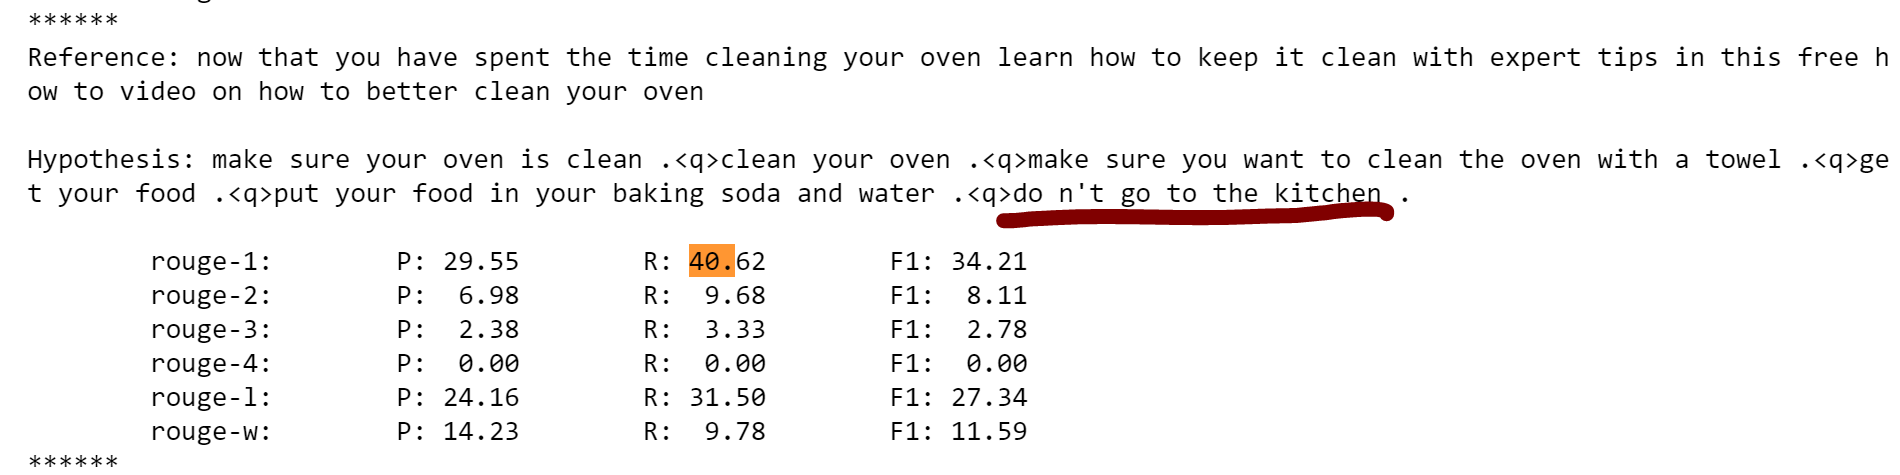
\includegraphics[width=\linewidth]{pic1.png}
  \caption{An example where ROUGE metric is confusing.}
  \label{fig:funnysummary}
\end{figure}

\section{Conclusion}
We are continuing to work on improving summarization for instructional videos, as measured by both ROUGE and human experts. By the end of the project, we hope to accomplish scores that are comparable to current SOTA, but more generalizable. We also plan to provide a more detailed analysis on correlations between features of a video (e.g. topic, length, number of likes) and the quality of summaries produced on our experiments, as well as a more detailed description of our expert evaluation process.


\section*{Broader Impact}

The contribution of our research is three-fold:
\begin{itemize}

\item We created and published a data set of how-to videos with time-tagged scripts, machine-generated summaries \footnote{https://github.com/alebryvas/berk266/ - it's not public repository yet, but we can provide access upon request}
\item We generalized  existing text summarization models to the scripts extracted from the videos [Sanabria et.al.]
\item We augmented ROUGE metrics [Chin-Yew Lin] for evaluation of the results with a framework for formalized expert assessment based on our research and criteria proposed by previous works \textit{[that's in work]}
\end{itemize}

At a high level, we hope that our analysis of transferability of summarization techniques from text to videos will have both practical and theoretical impacts by helping identify promising directions for future research.


\section*{References} 

{\bf We will allign the formatting of references for the final submission. Current list is accurate, but not standardized.}
\medskip



[1] Yang Liu, Mirella Lapata. Text Summarization with Pretrained Encoders.  \ (2019) URL. \url{https://arxiv.org/abs/1908.08345v2}

[2] Abigail See, Peter J. Liu, and Christopher D. Manning.\ (2017) Get to the point: Summarization with pointer-generator networks. In {\it Proceedings of the 55th Annual Meeting of the Association for Computational Linguistics \ (Volume 1: Long Papers)}, pages 1073-1083.

[3] Ilya Sutskever, Oriol Vinyals, and Quoc V Le. Sequence to sequence learning with neural networks.
 {\it Neural Information Processing Systems}, 2014. 

[4] Haoran Li, Junnan Zhu, Cong Ma, Jiajun Zhang, and Chengqing Zong. \ (2017). Multi-modal summarization for
asynchronous collection of text, image, audio and video. In {\it Proceedings of the 2017 Conference on Empirical
Methods in Natural Language Processing}, pages 1092–1102. Association for Computational Linguistics.

[5] Sanabria, R., Caglayan, O., Palaskar, S., Elliott, D., Barrault, L., Specia, L., and Metze, F. How2: A large-scale dataset for multimodal language understanding. {\it CoRR}, abs/1811.00347, 2018. URL. https://arxiv.org/abs/1811.00347

[6] Nenkova, A. (2005). Automatic text summarization of newswire: Lessons learned from the document understanding conference. In Proceedings of AAAI 2005, Pittsburgh, USA.

[7] Svore, K., Vanderwende, L., and Burges, C. (2007). Enhancing single-document summarization by combining RankNet and third-party sources. In Proceedings of the EMNLP-CoNLL, pages 448–457. [7, 8] 

[8] Yu-Hsiang Huang. Attention is all you need - pytorch. https://github.com/ jadore801120/attention-is-all-you-need-pytorch, 2018.

[9] Nima Sanjabi. Abstractive text summarization with attention-based mechanism. Master’s thesis, Universitat Politècnica de Catalunya, July 2018.

[10] Berna Erol, D-S Lee, and Jonathan Hull. 2003. Multimodal summarization of meeting recordings. In Multimedia and Expo, 2003. ICME’03. Proceedings. 2003 International Conference on, volume 3, pages III–25. IEEE.

[11] Dian Tjondronegoro, Xiaohui Tao, Johannes Sasongko, and Cher Han Lau. 2011. Multi-modal summarization of key events and top players in sports tournament videos. In Applications of Computer Vision (WACV), 2011 IEEE Workshop on, pages 471–478. IEEE

[12] Alexander M. Rush, Sumit Chopra, and Jason Weston. 2015. A neural attention model for abstractive sentence summarization. In Proceedings of the 2015 Conference on Empirical Methods in Natural Language Processing, pages 379–389. Association for Computational Linguistics.

[13] Shruti Palaskar, Jindrich Libovicky, Spandana Gella, Florian Metze. 2019. Multimodal Abstractive Summarization for How2 Videos. In Proceedings of the 57th Annual Meting of the Association for Computational Linguistics, pages 6587-6596. Association for Computational Linguistics.

[14] Antoine Miech, Dimitri Zhukov, Jean-Baptiste Alayrac, Makarand Tapaswi, Ivan Laptev, Josef Sivic. 2019. HowTo100M: Learning a Text-Video Embedding by Watching Hundred Million Narrated Video Clips. In ICCV 2019. https://arxiv.org/abs/1906.03327.



\end{document}
